\documentclass[12pt,twoside]{report}
\usepackage{graphicx}
\usepackage{alphalph}
\usepackage{subcaption}
\usepackage[a5paper,margin=1cm]{geometry}
\renewcommand*{\thesubfigure}{(\arabic{subfigure})}
\begin{document}
\begin{figure}
\centering
\begin{subfigure}[b]{0.20\textwidth}
\centering

\includegraphics[width=\textwidth]{../../trajectories/73.png}
\caption{Id:73}
\end{subfigure}
\begin{subfigure}[b]{0.20\textwidth}
\centering

\includegraphics[width=\textwidth]{../../trajectories/166.png}
\caption{Id:166}
\end{subfigure}
\begin{subfigure}[b]{0.20\textwidth}
\centering
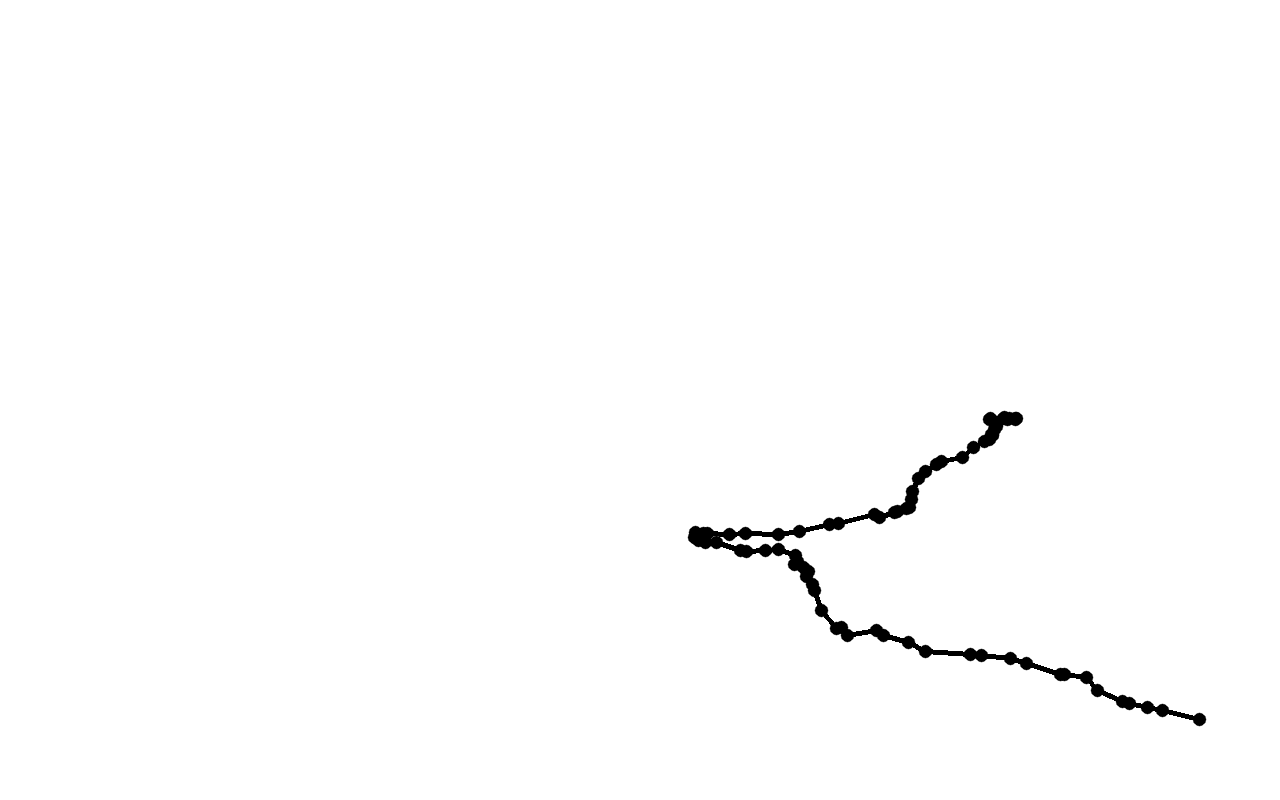
\includegraphics[width=\textwidth]{../../trajectories/287.png}
\caption{Id:287}
\end{subfigure}
\begin{subfigure}[b]{0.20\textwidth}
\centering
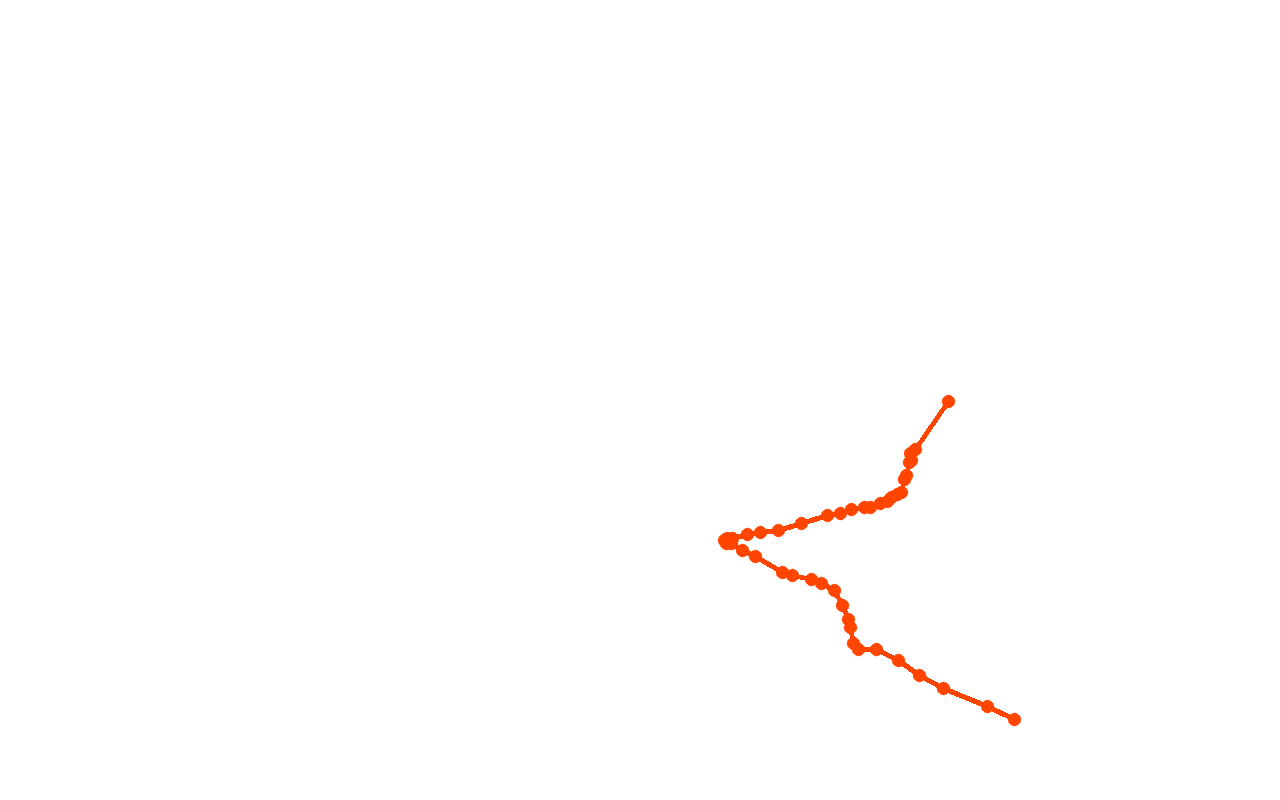
\includegraphics[width=\textwidth]{../../trajectories/548.png}
\caption{Id:548}
\end{subfigure}
\begin{subfigure}[b]{0.20\textwidth}
\centering

\includegraphics[width=\textwidth]{../../trajectories/612.png}
\caption{Id:612}
\end{subfigure}
\begin{subfigure}[b]{0.20\textwidth}
\centering

\includegraphics[width=\textwidth]{../../trajectories/768.png}
\caption{Id:768}
\end{subfigure}
\end{figure}
\end{document}